\documentclass[11pt,a4paper]{article}

% --- Core Packages ---
\usepackage[utf8]{inputenc}
\usepackage[T1]{fontenc}
\usepackage{lmodern}
\usepackage{microtype}
\usepackage[margin=1in]{geometry}
\usepackage{amsmath,amssymb,amsfonts,amsthm}
\newtheorem{definition}{Definition}
\usepackage{booktabs}
\usepackage{graphicx}
\usepackage{tabularx}
\usepackage{multirow}
\usepackage{makecell}
\usepackage{array}
\usepackage{enumitem}
\usepackage{xcolor}
\usepackage{hyperref}
\usepackage{tikz}
\usetikzlibrary{shapes.geometric,arrows.meta,positioning,calc,fit,backgrounds}
\usepackage{pgfplots}
\pgfplotsset{compat=1.17}
\usepackage{caption}
\usepackage{subcaption}
\usepackage{algorithm}
\usepackage{algorithmic}

% --- Color Definitions & Hyperref Setup ---
\definecolor{agriTeal}{RGB}{0,102,102}
\definecolor{agriDark}{RGB}{24,43,49}
\definecolor{safetyRed}{RGB}{180,40,40}
\definecolor{factBlue}{RGB}{28,90,160}
\definecolor{cropGreen}{RGB}{34,120,60}
\definecolor{lightGray}{RGB}{248,249,250}
\definecolor{borderGray}{RGB}{200,205,210}

\hypersetup{
    colorlinks=true,
    linkcolor=agriTeal,
    citecolor=factBlue,
    urlcolor=agriTeal,
    pdftitle={Evaluating Detection-Gated Deterministic Routing for Fail-Closed Agricultural Advisory under Low-Connectivity Constraints},
    pdfauthor={Raiyaan Reza}
}

\usepackage{fancyhdr}
\usepackage{authblk}
\usepackage{titlesec}

% --- Typography & Section Styling ---
\titleformat{\section}{\large\bfseries\color{agriDark}}{\thesection.}{0.6em}{}
\titleformat{\subsection}{\normalsize\bfseries\color{agriDark}}{\thesubsection}{0.6em}{}
\titleformat{\subsubsection}{\small\bfseries\color{agriDark}}{\thesubsubsection}{0.6em}{}
\titlespacing*{\section}{0pt}{1.2em}{0.4em}
\titlespacing*{\subsection}{0pt}{0.9em}{0.3em}

% --- Running Headers & Footers ---
\pagestyle{fancy}
\fancyhf{}
\fancyhead[L]{\small\textit{Detection-Gated Deterministic Routing for Agricultural Advisory}}
\fancyhead[R]{\small\textit{Reza}}
\fancyfoot[C]{\thepage}
\renewcommand{\headrulewidth}{0.4pt}
\renewcommand{\footrulewidth}{0pt}

% --- Custom Column Types ---
\newcolumntype{L}[1]{>{\raggedright\arraybackslash}p{#1}}
\newcolumntype{C}[1]{>{\centering\arraybackslash}p{#1}}
\newcolumntype{R}[1]{>{\raggedleft\arraybackslash}p{#1}}
\newcolumntype{Y}{>{\raggedright\arraybackslash}X}

% --- Title & Author Metadata ---
\title{\vspace{-1.5em}\LARGE\bfseries\color{agriDark} Evaluating Detection-Gated Deterministic Routing for Fail-Closed Agricultural Advisory under Low-Connectivity Constraints\vspace{0.3em}}

\author{\textbf{Raiyaan Reza}\thanks{Corresponding author. Email: \texttt{raiyanreza.contact@gmail.com}}}
\affil{\small Independent Agricultural AI Researcher \& Systems Engineer, Dhaka, Bangladesh}

\date{}

\begin{document}

\maketitle
\thispagestyle{plain}

\vspace{-1.0em}
\begin{quote}
\small
\noindent\textbf{\color{agriDark}\large Abstract}\vspace{0.4em}

\noindent
Low-resource agricultural advisory combines safety-critical content constraints with language, connectivity, and delivery limits. A recommendation can be unsafe when chemical identity, formulation, dose, interval, pre-harvest interval, or crop applicability is wrong, even when its wording is fluent. We evaluate an architecture for bounded Bengali agricultural workloads that conditions deterministic fact lookup on structured crop/disease metadata. Detection-Gated Deterministic Routing (DGDR) gates a fact-base partition and reserves text retrieval and LLM generation for fallback paths. A typed 11-slot contract certifies a candidate only when required relations are jointly supported by one authoritative record; otherwise it abstains or escalates. In offline evaluations, the gate reduced the candidate partition from 2{,}135 nodes to a mean of 516.4 at $\gamma=0.80$ and recorded 3.15\% misrouting. In a 5{,}000-query workload, 61.52\% of requests reached zero-LLM terminal paths, including safety handling and refusal. The dialect-hazard suite measured coverage rising from 42.9\% to 89.8\% for regional queries; coverage is not correctness. Deterministic GSM composition preserved the selected safety-critical slots in 1{,}000 tested tuples, while an LLM-composed control incurred a 64.4\% critical-hazard rate. Across separately evaluated safety suites, zero dangerous acceptances were observed, with suite-specific Wilson upper bounds. The E25 comparison records a trade-off: joint accuracy was 78.4\% for the lightweight classifier versus 94.2\% for the comparison LLM. These results support reduced text and LLM dependence for the tested workloads, but do not establish universal safety, field performance, or deployment readiness.

\vspace{0.8em}
\noindent\textbf{Keywords:} Agricultural expert systems, edge AI, on-device inference, network-resilient advisory, ICT4D, deterministic retrieval gating, relational verification, agrochemical safety, digital agricultural extension.
\end{quote}

\vspace{0.8em}
\hrule
\vspace{1.2em}


% -------------------------------------------------------------------------
% 1. INTRODUCTION
% -------------------------------------------------------------------------
\section{Introduction}
\label{sec:introduction}

Consider a farmer thirty kilometres outside Kurigram at the start of the boro season. She holds a sub-\$120 Symphony or Walton handset, the network shows a flickering 2G indicator, and the query she types mixes Bangla script with romanised Chittagonian words for a leaf symptom she cannot name precisely. If an automated advisory replies with a fluent Bengali paragraph that names the right chemical but the wrong dose interval, omits the pre-harvest interval, or swaps the formulation with a neighbouring record, the consequence is not a lower BLEU score. It is a burnt plot, a poisoned spray operator, or contaminated water. Correctness therefore depends on the joint binding of chemical identity, formulation, dose interval, unit, spray volume, interval, pre-harvest interval, crop, growth stage, and regulatory polarity to \emph{one} authoritative record. A system must control retrieval, generation, certification, and delivery as separate failure surfaces, because each can silently produce that wrong binding.

Bangladesh makes this systems problem concrete. The Bangladesh Bureau of Statistics reports more than 16 million farming households~\cite{bbs2019}, while the Department of Agricultural Extension reports an officer-to-household ratio above 1:1{,}000~\cite{dae2021}. The national Krishi Call Center at 16123 exists as a defined institutional escalation endpoint. Its existence establishes where an unresolved case can be referred; it does not establish referral access, follow-through, or farmer benefit. In this setting a cloud-only chatbot, a text-only retriever, and a subscription priced at \$2.30 per thousand queries are each individually plausible in a laboratory, and each individually fragile in the field.

The three fragilities are distinct, so they must be evaluated as distinct endpoints. A cloud model can generate a plausible answer without binding its chemical attributes to the same source record. Text retrieval can rank a formal Bengali passage above a colloquial or romanised query. A network or message-length constraint can prevent a certified field from reaching the user. A useful evaluation therefore reports evidence binding, language handling, and delivery as separate measurements rather than collapsing them into answer accuracy.

\subsection{Measured Constraints and Bounded Hypothesis}
\label{subsec:three_dependencies}
\begin{enumerate}[leftmargin=1.8em]
    \item \textbf{Treatment and evidence risk.} Our prior benchmark found treatment correctness below 44\% for every tested zero-shot baseline and a residual chemical-hallucination rate even when evidence was supplied.\footnote{Authoritative artifact: the KrishokChat benchmark PDF in \texttt{paper/done papers/}.} These measurements motivate explicit evidence binding; they do not show that every LLM or cloud system fails in the same way.
    \item \textbf{Dialect-sensitive retrieval.} The prior retrieval study measured lower dense-retrieval performance on regional queries than on formal Bengali.\footnote{Authoritative prior-paper artifact: \texttt{paper/done papers/AgriTrust.pdf}.} In the present evaluation, Hit@1, coverage, and joint certification are reported as different endpoints. The image-conditioned path is tested for reduced text dependence, not as evidence that dialect or orthographic variation is resolved.
    \item \textbf{Network and channel limits.} E14 models packet loss and latency, so its delivery result is a simulation rather than a field measurement. E15 tests message composition within the GSM-03.38 budget. Neither experiment measures mobile access, carrier reliability, helpline use, or farmer outcomes.
\end{enumerate}

\noindent These premises motivate a bounded systems hypothesis: for a specified Bengali fact base and query workload, reliable crop/disease metadata can reduce dependence on text retrieval and LLM inference by selecting a narrower deterministic search path. The same design introduces perception and misrouting risks, so the evaluation must measure fallback, coverage, Hit@1, and misrouting rather than infer safety from routing alone.

\begin{quote}
\itshape For the evaluated workload, structured metadata may reduce text and LLM dependence when deterministic lookup is conditioned on explicit fallback and certification rules. This hypothesis does not extend the result beyond the specified workload.
\end{quote}

\subsection{Approach and Contributions}
\label{subsec:contributions}
We evaluate DGDR as a systems architecture rather than as a replacement for all language processing. On-device crop/disease metadata and a compact intent classifier select a fact-base partition for an image-conditioned path. If confidence is insufficient or deterministic traversal finds no supported relation, the system falls back to text-first retrieval, grounded generation, or abstention. A fail-closed typed relational verifier certifies an advisory only when the required slots bind jointly to one authoritative institutional record. This contract assumes correct parsing, current authoritative records, complete required fields, no bypass path, and tested implementation; it cannot repair an incorrect classifier or an incomplete fact base.

\begin{figure}[t]
\centering
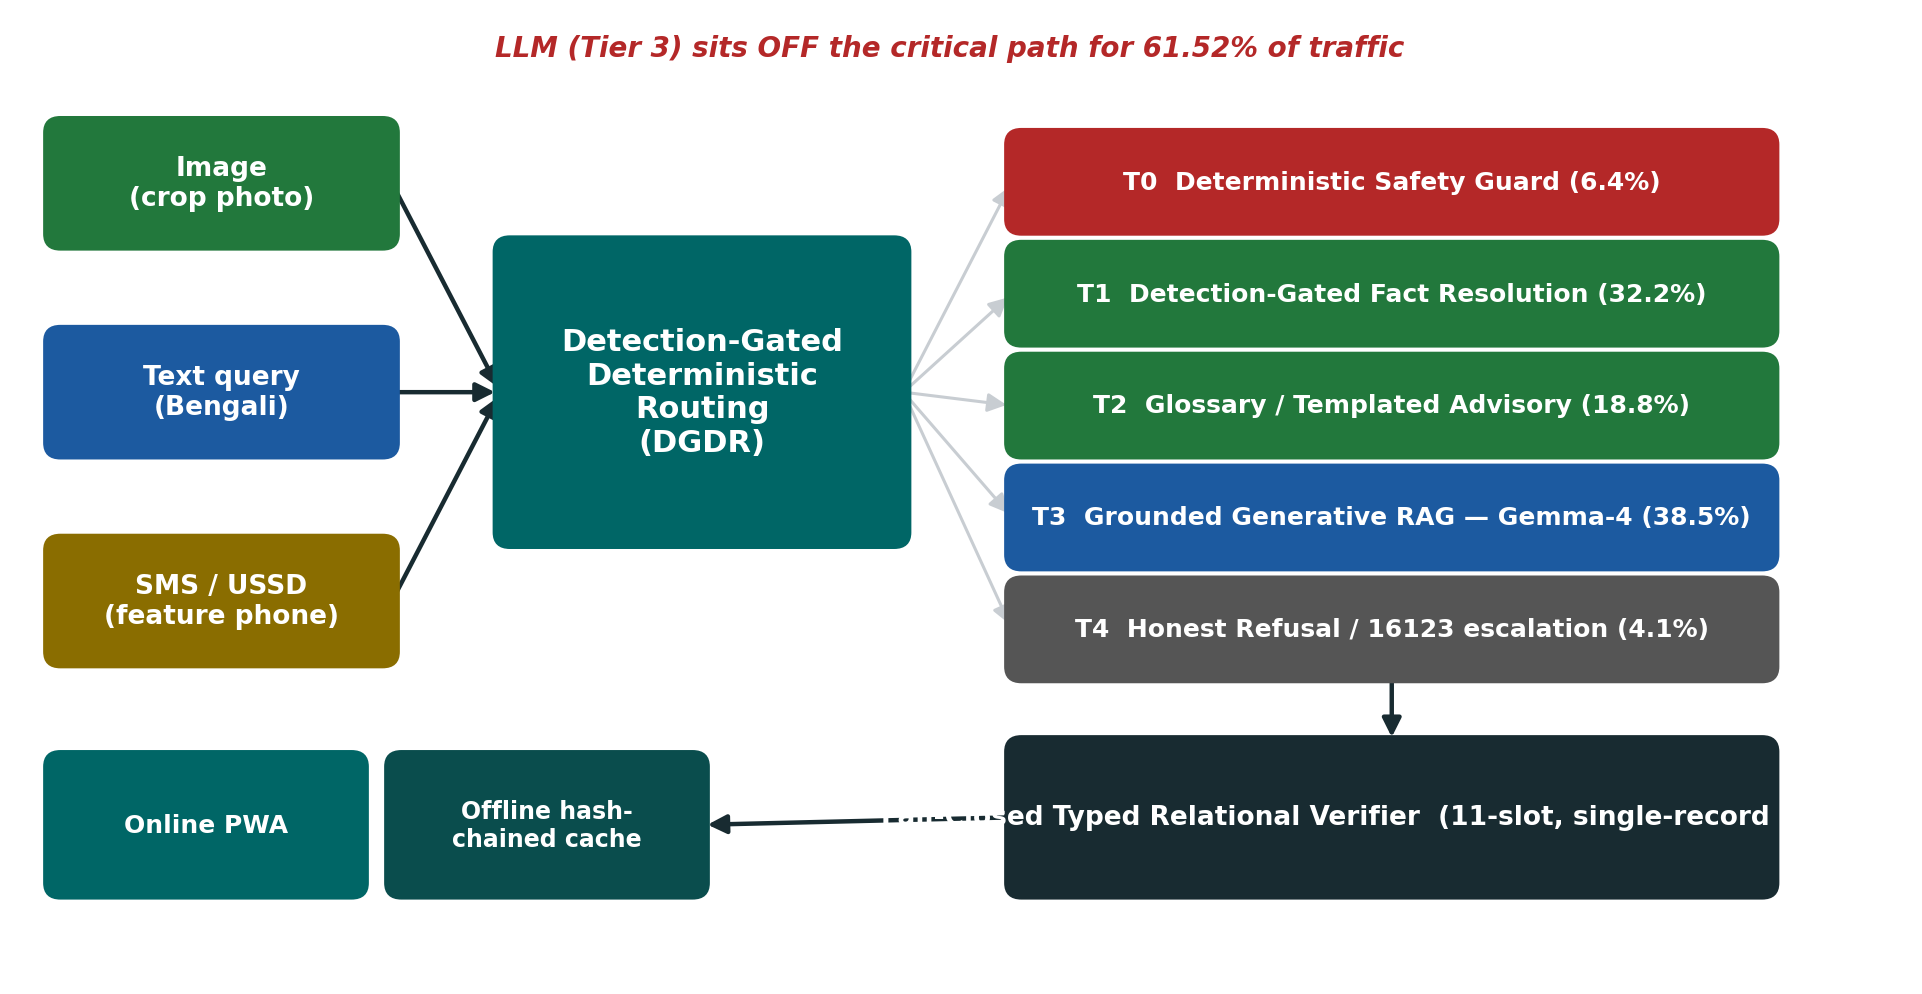
\includegraphics[width=\textwidth]{figures/fig_1_architecture.png}
\vspace{-0.5em}
\caption{\textbf{Evaluated edge--cloud architecture.} Image, text, and SMS inputs enter Detection-Gated Deterministic Routing. Structured metadata selects a fact-base partition when the gate accepts; otherwise the system uses an explicit text-retrieval fallback or abstains. The production path and offline research components are evaluated separately, and certified candidates pass through the typed relational verifier before delivery through online, cached, or GSM channels.}
\label{fig:architecture}
\vspace{-0.5em}
\end{figure}

Our contributions are:
\begin{enumerate}[label=\textbf{C\arabic*.}]
    \item \textbf{Detection-Gated Deterministic Routing (DGDR).} Structured crop/disease metadata gates deterministic lookup before text retrieval, collapsing the candidate partition from 2{,}135 nodes to 516.4 and reducing the measured dependence on formal Bengali. The design reports its threshold ($\gamma=0.80$), fallback share (13.55\%), and misrouting rate (3.15\%) rather than claiming dialect immunity (E17, E19, E21, E25).
    \item \textbf{A conditional fail-closed certification contract.} An 11-slot typed tuple, single-record joint binding, and abstention or escalation when required relations are unsupported. The contract is evaluated as a bounded test property across adversarial, generator, retrieval, dialect, and channel suites (E02--E05, E07--E13, E21--E22).
    \item \textbf{A network-resilient offline-first cache.} A hash-chained fact pack with signed invalidation that sustains delivery under emulated 2G/Edge loss and with tamper-evident updates (791\,B delta). The result is a software/simulation measurement, not a live-carrier claim (E14, E23).
    \item \textbf{A deterministic GSM-160 gateway.} A fixed template that preserves selected safety-critical slots within the 160-character budget, compared with an LLM-composed control that incurred a 64.4\% critical-hazard rate and 36.4\% injection leakage into outbound SMS (E15, E22).
    \item \textbf{A bounded telecom-economic scenario.} A localised cost model using real BTRC A2P tariffs (0.25\,BDT/SMS), measured tier mix (61.52\% zero-LLM terminal handling), and stated hosting and workload assumptions. National projections are reported as scenarios, not as audited spend (E09, E18, E20).
    \item \textbf{A measurable knowledge-growth loop and expert review.} A demand-ranked authoring intervention that closed a 55-query Chili Anthracnose gap in 18\,min (3.06 queries/min) and a double-blind review by three agronomists on 200 responses (Gwet's AC$_{1}=0.862$). Both are bounded observations, not general productivity or field-benefit claims (E13, E24, E26).
\end{enumerate}

\subsection{Research Questions}
\begin{itemize}[leftmargin=1.8em]
    \item \textbf{RQ1 (Routing):} Under the evaluated query construction, does structured detection metadata reduce the candidate search space and change retrieval or coverage metrics relative to text-first lookup? (E17, E19, E21)
    \item \textbf{RQ2 (Dependency):} What proportion of the specified workload reaches a zero-LLM terminal path, and how do its measured latency and modeled serving cost compare with the baseline? (E9, E18, E20)
    \item \textbf{RQ3 (Safety behavior):} In separately evaluated generator, retrieval, dialect, and channel suites, how often does the certification path accept a harmful candidate, and what confidence bounds apply? (E02--E05, E07--E13, E21--E22)
    \item \textbf{RQ4 (Network):} Under simulated network profiles, how does offline-first caching change delivery success and cache latency, and what stale-record behavior is observed? (E14, E23)
    \item \textbf{RQ5 (Channel):} Does deterministic template composition preserve selected safety-critical fields within the GSM-03.38 budget, and can tested injection payloads survive into outbound SMS? (E15, E22)
    \item \textbf{RQ6 (Operations):} What do the specified local-cost assumptions imply for serving scenarios, and how much demand coverage did one targeted fact-authoring intervention add? (E20, E24)
\end{itemize}

\noindent\textbf{Structure.} Section~\ref{sec:related_work} reviews adjacent agricultural, verification, low-resource, vision, and ICT4D systems. Section~\ref{sec:architecture} presents the deployment context and DGDR. Section~\ref{sec:algorithms} formalises routing and certification. Section~\ref{sec:experiments} defines the production, research-harness, simulated, and modeled evidence. Section~\ref{sec:results} reports the named evaluations by research question. The remaining sections discuss failure modes, implications, limitations, reproducibility, and conclusions.


% -------------------------------------------------------------------------
% 2. RELATED WORK
% -------------------------------------------------------------------------
\section{Related Work}
\label{sec:related_work}

We position the system across six connected literatures: agricultural advisory and extension, RAG and evidence verification, selective answering, Bengali and dialect retrieval, edge vision, and ICT4D delivery. The comparison separates input channel, grounding, evaluation endpoint, escalation, and deployment evidence. It does not treat a missing report in one paper as evidence that no comparable system exists.

\subsection{Agricultural Advisory and Extension Systems}
Rule-based expert systems, ontologies, and diagnostic decision trees encode extension guidance with explicit decision paths~\cite{liao2005expert, prasad2008hybrid}. CABI Plantwise shows how pest-management knowledge can be organized as structured decision guidance~\cite{cabi2020plantwise}. Farmer.Chat extends retrieval-grounded agricultural advice to multilingual conversational channels and reports service-level and user-facing evaluations~\cite{farmerchat2024}. KrishokBondhu represents a Bengali voice-RAG line, while AIEP represents a voice-first, modular extension architecture~\cite{krishokbondhu2025,aiep2026}. A translation-centric Bengali system instead places an intermediate English retrieval step between the farmer and the corpus~\cite{crosslingualbengali2026}.

Our prior KrishokChat benchmark measures Bengali agricultural generation and treatment limitations, while the accompanying AgriTrust artifact measures retrieval and provenance behavior.\footnote{The authoritative prior-paper PDFs are stored in \texttt{paper/done papers/}; no public identifier is asserted here.} These systems differ in channel, grounding, and evaluation scope. \textit{Bounded gap:} this paper evaluates the additional interaction between metadata-gated routing, typed certification, and constrained delivery for a specified Bengali workload.

\subsection{RAG, Claim Verification, and Safety}
RAG supplies retrieved passages to a generator for knowledge-intensive tasks~\cite{lewis2020rag, gao2023ragsurvey}. FEVER established sentence-level entailment as a fact-verification task~\cite{thorne2018fever}; FActScore decomposes long-form outputs into atomic facts~\cite{min2023factscore}; and FacTool uses tools for factuality checks~\cite{chern2023factool}. Other work studies retrieval hallucination~\cite{ren2024investigating, varshney2023stitch}, fine-grained verification~\cite{malladi2024fine}, automated RAG evaluation~\cite{es2024ragas}, and self-reflective retrieval~\cite{asai2024selfrag}.

The reviewed taxonomy also includes RAGChecker, RT4CHART, VeriCite, and medical verifiers that add claim decomposition, attribution, or domain relations~\cite{rt4chart2026}. These approaches distinguish retrieval quality, citation quality, and claim support. \textit{Bounded gap:} the present work tests whether an agrochemical candidate can be certified only when its required typed relations are jointly supported by one authoritative record.

\subsection{Selective Answering and Abstention}
Selective classification formalizes a reject option when a model lacks sufficient confidence~\cite{geifman2017selective, geifman2019selectivenet}. Calibration methods estimate whether confidence tracks correctness~\cite{guo2017calibration}, while selective question answering addresses domain shift~\cite{kamath2020selective}. Conformal methods provide coverage-oriented prediction sets under stated assumptions~\cite{angelopoulos2023conformal, romano2020classification}. Language-model uncertainty work studies whether models can identify knowledge limits~\cite{kadavath2022language}; related systems in the reviewed literature include ConfRAG, CRAG, and Self-RAG.

RefusalBench and related work show why refusal should be measured rather than assumed~\cite{refusalbench2025}. In this paper, abstention is an operating policy: unsupported fields produce refusal or escalation. It is not treated as proof that an accepted advisory is agronomically correct. \textit{Bounded gap:} the evaluation couples abstention to a typed, single-record certification contract and reports coverage separately from joint accuracy and slot completeness.

\subsection{Bengali, Dialect, and Low-Resource Retrieval}
Low-resource retrieval depends on both representation and query form. The AgriTrust artifact shows that Bengali agricultural retrieval varies by query register and that provenance-preserving evaluation is needed. Our prior benchmark likewise treats farmer-language transfer as distinct from standard written Bengali. The reviewed Bengali literature includes normalization resources for regional and romanized input, but normalization does not by itself establish retrieval correctness, safety behavior, or agronomic adequacy.

The present study therefore distinguishes text-first Hit@1 from image-conditioned coverage, joint certification, and dangerous acceptance. \textit{Bounded gap:} it tests reduced text dependence on the evaluated image-conditioned path without treating dialect or language variation as resolved.

\subsection{Vision and Edge Agricultural Computing}
Agricultural vision research commonly separates crop or disease classification from subsequent advisory generation. Hierarchical classifiers can narrow the diagnostic task, while vision-to-RAG systems connect a predicted disease label to textual guidance. The artifacts used here report \texttt{task: classify}; they do not localize lesions or supply bounding-box evidence.

The paper therefore treats crop/disease metadata as a routing signal and evaluates fallback and misrouting rather than presenting a new detector. \textit{Bounded gap:} the evaluation asks whether structured visual metadata can reduce text and LLM dependence while exposing the perception errors introduced by that gate.

\subsection{ICT4D Channels and Offline Service Delivery}
SMS, IVR, USSD, voice interfaces, and human extension services address access conditions that differ from web chat. Offline-first designs add local data and update mechanisms, but delivery success, stale-record handling, message fidelity, and human escalation are separate system properties. This paper uses 16123 as a defined Bangladesh escalation endpoint, not as evidence of referral uptake. Its GSM and network findings come from software tests and simulation, not carrier operation or field deployment. \textit{Bounded gap:} the evaluation connects deterministic safety-field composition and cache provenance to low-connectivity delivery without claiming adoption, trust, or farmer outcomes.


% -------------------------------------------------------------------------
% 3. SYSTEM ARCHITECTURE
% -------------------------------------------------------------------------
\section{System Architecture}
\label{sec:architecture}

KrishokChat is a single-process FastAPI backend paired with an offline-capable Next.js Progressive Web Application (PWA) and an SMS/USSD gateway. For this paper, the term ``architecture'' refers to the evaluated research path and its interfaces; it does not imply that every research component is active in the production runtime.

\begin{quote}\small
\textbf{Evidence boundary.} The production application, the offline experiment harness, and the proposed deployment architecture are separate objects. Production facts are established by the application audit; E14--E26 are research-layer measurements, simulations, or projections. The results section labels these distinctions explicitly.
\end{quote}

\subsection{Deployment Context and Constraint Budget}
\label{subsec:constraints}
The design is disciplined by the physical realities of rural Bangladeshi deployment. Table~\ref{tab:constraints} states the binding constraints; every architectural choice below is traceable to a row.

\begin{table}[t]
\centering
\small
\caption{\textbf{Physical deployment constraint budget.} Each constraint drives a concrete design decision, validated in the indicated layer.}
\label{tab:constraints}
\begin{tabularx}{\textwidth}{@{} L{3.4cm} L{3.6cm} Y @{}}
\toprule
\textbf{Constraint} & \textbf{Budget} & \textbf{Design response (layer)} \\
\midrule
Device RAM (low-end) & $\leq$ 100\,MB working set & INT8 ONNX vision at 42.5\,MB RAM (E9) \\
On-device model size & per-model footprint reported & 5.90\,MB crop classifier; 1.25\,MB intent artifact (E9, E25) \\
GSM message length & 160 chars (GSM 03.38) & Deterministic template, 102--115 chars (E15) \\
Rural packet loss & up to 30\% (severe 2G) & Offline-first hash-chained cache (E14, E23) \\
A2P SMS tariff (BTRC) & 0.25 BDT / message & Tier-gated SMS only on fallback (E20) \\
Officer:farmer ratio & $>$ 1:1{,}000 & Selective abstention routes only residual load to humans (E6) \\
\bottomrule
\end{tabularx}
\vspace{-0.5em}
\end{table}

\subsection{Detection-Gated Deterministic Routing (DGDR)}
\label{subsec:dgdr}
The architectural focus is the use of on-device classification metadata as \emph{retrieval-gating structure}. When a farmer submits an image, an INT8 crop classifier and, where applicable, a disease classifier produce a $\langle$crop, pathogen$\rangle$ label with a confidence score. A 1.25\,MB character-$n$-gram artifact provides optional intent features. At the selected gate $\gamma=0.80$, the fact-base query is restricted to the crop/pathogen-conditioned partition; E17 reports a mean of 516.4 nodes instead of 2{,}135 ($-75.6\%$) and a 3.15\% misrouting rate. This path does not require the query to be expressed in formal Bengali, but it remains exposed to classifier error and incomplete image/query pairing. Below the gate, or when no image is supplied, the system follows the text-first fallback or abstains. The verifier does not repair an incorrect crop or pathogen label; it only controls whether the resulting candidate satisfies the encoded evidence contract.

\begin{figure}[t]
\centering
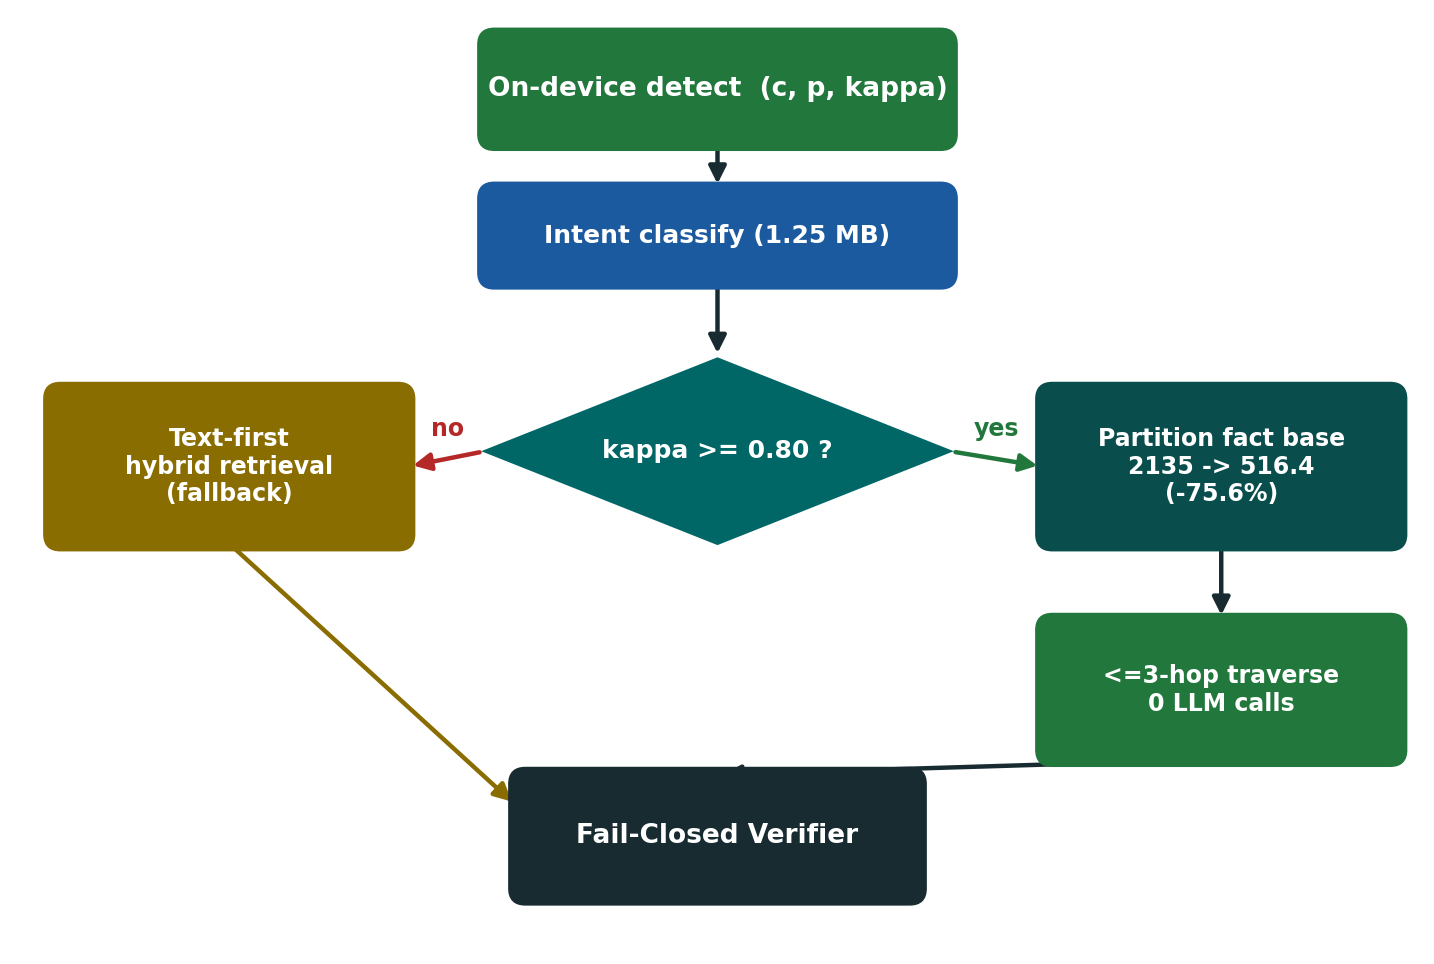
\includegraphics[width=0.86\textwidth]{figures/fig_2_dgdr.png}
\vspace{-0.5em}
\caption{\textbf{DGDR decision flow.} On-device classification at confidence $\geq 0.80$ gates the fact-base partition (2{,}135 $\to$ 516.4 nodes); below threshold, or without an image, control falls back to text-first retrieval. All candidate paths converge on the evaluated certification contract.}
\label{fig:dgdr}
\vspace{-0.5em}
\end{figure}

\subsection{Five-Tier Resolution Ladder}
\label{subsec:tiers}
Queries are processed sequentially to prioritise deterministic handling and limit LLM use. The E18 workload mix is shown in parentheses. The percentages are terminal-path shares, not agronomic correctness rates:
\begin{itemize}[leftmargin=1.5em]
    \item \textbf{Tier 0 --- Deterministic Safety Guard} (6.4\%): pre-retrieval screening of banned substances (Paraquat, Endosulfan, Monocrotophos), self-harm/poisoning hazards, and prompt injections, with a calm redirect to the Krishi Call Center (16123).
    \item \textbf{Tier 1 --- Detection-Gated Fact Resolution} (32.22\%): sub-millisecond lookup against verified BARI/BRRI fact tuples for exact dose, formulation, and PHI (0 LLM calls).
    \item \textbf{Tier 2 --- Glossary / Templated Advisory} (18.82\%): rule-based assembly of stage tasks and IPM guidance from verified crop calendars (0 LLM calls).
    \item \textbf{Tier 3 --- Grounded Generative RAG} (38.48\%): hybrid retrieval feeding a fine-tuned Gemma-4 4-bit model, subjected to post-generation relational verification.
\item \textbf{Tier 4 --- Honest Refusal} (4.08\%): explicit refusal and helpline escalation when the tested policy does not select a supported path.
\end{itemize}
Tiers 0--2 and 4 together account for \textbf{61.52\%} zero-LLM terminal handling. Tiers 1 and 2 alone account for 51.04\% of the workload as deterministic advisory paths; T0 and T4 are safety handling and refusal, respectively.

\subsection{The 11-Slot Relational Schema and Fail-Closed Certification}
\label{subsec:schema}
An agrochemical claim is a typed 11-slot relational tuple (permissible dosage captured by the composite interval $[d_{\min}, d_{\max}]$):
\begin{equation}
\label{eq:claim_tuple}
\mathcal{C} = \langle c, p, s, a, f, [d_{\min}, d_{\max}], u, v, \tau, \phi, \rho \rangle
\end{equation}
comprising host crop $c$, pathogen $p$, growth stage $s$, active ingredient $a$, formulation $f$, dosage bounds $[d_{\min}, d_{\max}]$, unit $u$, solvent volume $v$, spray interval $\tau$, pre-harvest interval $\phi$, and regulatory polarity $\rho \in \{+1,-1\}$. The research contract requires $\rho=+1$, successful extraction of required fields, a single evidence record $e$ that entails all required slots, and a confidence score above a development-selected threshold $\theta^*$:
\begin{equation}
\label{eq:certification_contract}
\pi(x) = \begin{cases}
\text{CERTIFY}(\hat{y}) & \text{if } \rho{=}{+}1 \,\land\, \exists e \in \mathcal{E}: \text{Entails}(e,\mathcal{C}_{\hat{y}}) \,\land\, g(x) \ge \theta^* \\
\text{ESCALATE}(16123) & \text{if } \rho{=}{-}1 \,\lor\, \text{IsCrisis}(x) \\
\text{ABSTAIN} & \text{otherwise}
\end{cases}
\end{equation}
This is a conditional contract, not a universal safety theorem. It is meaningful only when parsing is correct, the evidence record is authoritative and current, the implementation cannot be bypassed, and the required fields are present. The experiments therefore report observed dangerous acceptance in defined suites rather than claiming zero risk in the deployment population.

\subsection{Edge Client, SMS Gateway, and Human Escalation}
\label{subsec:client}
The PWA can use INT8 ONNX classifiers and a local fact pack for the evaluated edge path. Low-confidence images undergo client-side dimension clamping ($\leq 1024$\,px), EXIF stripping, and WebP compression before upload. For feature-phone delivery, the research gateway renders a certified tuple into a GSM-160 template (Section~\ref{subsec:e15}); E15 and E22 test composition, not live carrier delivery. The defined escalation endpoint is the Krishi Call Center at 16123, but referral follow-through and operator workload were not measured.




% -------------------------------------------------------------------------
% 4. CORE ALGORITHMS
% -------------------------------------------------------------------------
\section{Core Algorithms}
\label{sec:algorithms}

We formalise the four mechanisms evaluated in this paper: detection-gated resolution (Algorithm~\ref{alg:dgdr}), typed certification (Algorithm~\ref{alg:verifier}), cache invalidation (Algorithm~\ref{alg:cache}), and GSM template composition (Algorithm~\ref{alg:sms}).

\begin{algorithm}[t]
\caption{Detection-Gated Deterministic Resolution}
\label{alg:dgdr}
\begin{algorithmic}[1]
\REQUIRE Query $x$; optional image $I$; fact base $\mathcal{F}$ ($2{,}135$ nodes); gate $\gamma{=}0.80$
\ENSURE Candidate $\hat{y}$, fallback signal, or abstention
\IF{$I \ne \varnothing$}
    \STATE $(c, p, \kappa) \gets \textsc{ClassifyOnDevice}(I)$ \hfill // classification, not localization
\ELSE
    \STATE $(c,p,\kappa) \gets (\varnothing,\varnothing,0)$
\ENDIF
\STATE $\iota \gets \textsc{IntentClassify}(x)$ \hfill // optional 1.25\,MB char-$n$-gram artifact
\IF{$\kappa \ge \gamma$}
    \STATE $\mathcal{F}_{\text{sub}} \gets \textsc{Partition}(\mathcal{F}, c, p)$
    \STATE $\hat{y} \gets \textsc{DeterministicTraverse}(\mathcal{F}_{\text{sub}}, \iota, \text{maxhops}{=}3)$
    \IF{$\hat{y} \ne \varnothing$}
        \STATE $v \gets \mathrm{Verify}(\hat{y},\mathcal{F}_{\mathrm{sub}})$
        \IF{$v=1$}
            \RETURN $\hat{y}$ \hfill // deterministic candidate accepted by the contract
        \ENDIF
    \ENDIF
\ENDIF
\STATE $\mathcal{R} \gets \textsc{TextFirstRetrieve}(x)$ \hfill // explicit fallback path
\IF{$\mathcal{R}=\varnothing$}
    \RETURN \textsc{Abstain}
\ENDIF
\STATE $\hat{y} \gets \textsc{GroundedGenerate}(x, \mathcal{R})$
\RETURN $\textsc{Verify}(\hat{y},\mathcal{R})$ \hfill // Algorithm~\ref{alg:verifier}
\end{algorithmic}
\end{algorithm}

\begin{algorithm}[t]
\caption{Fail-Closed Typed Relational Verification}
\label{alg:verifier}
\begin{algorithmic}[1]
\REQUIRE Candidate $\hat{y}$; evidence set $\mathcal{E}$; frozen threshold $\theta^*$; slot schema (Eq.~\ref{eq:claim_tuple})
\ENSURE $\textsc{Certify}$, $\textsc{Escalate}$, or $\textsc{Abstain}$
\STATE $\mathcal{C} \gets \mathrm{ExtractSlots}(\hat{y})$ \hfill // parse into 11-slot tuple; failure returns null
\IF{$\mathcal{C}=\varnothing$}
    \RETURN \textsc{Abstain}
\ENDIF
\IF{$\rho(\mathcal{C}) = -1$}
    \RETURN $\mathrm{ESCALATE}(16123)$ \hfill // banned/restricted: fail closed
\ENDIF
\STATE $\text{bound} \gets \mathrm{true}$
\FORALL{slot $\sigma \in \{c,p,s,a,f,[d_{\min},d_{\max}],u,v,\tau,\phi\}$}
    \IF{$\nexists\, e \in \mathcal{E}: \mathrm{Entails}(e, \sigma)$}
        \STATE $\text{bound} \gets \mathrm{false}$; \textbf{break} \hfill // any unbound safety slot fails closed
    \ENDIF
\ENDFOR
\IF{$\text{bound} \wedge \exists\, e^{\star}\!\in\!\mathcal{E}\; \mathrm{EntailsAll}(e^{\star},\mathcal{C}) \wedge g(\hat{y}) \ge \theta^*$}
    \RETURN $\mathrm{CERTIFY}(\hat{y})$
\ELSE
    \RETURN \textsc{Abstain} \hfill // default action is refusal, not delivery
\ENDIF
\end{algorithmic}
\end{algorithm}

\begin{algorithm}[t]
\caption{Hash-Chained Cache Invalidation}
\label{alg:cache}
\begin{algorithmic}[1]
\REQUIRE Local fact pack $P$, update manifest $U$, expected corpus version $v$
\ENSURE Updated pack or safe removal of invalid records
\IF{$U.version \ne v$}
    \RETURN $\mathrm{REJECT\_UPDATE}$
\ENDIF
\FORALL{record $r \in P$}
    \IF{$\mathrm{SHA256}(r) \ne r.hash \OR r.hash \in U.deprecated\_hashes$}
        \STATE $\mathrm{Purge}(r)$
    \ENDIF
\ENDFOR
\STATE $\mathrm{VerifyChain}(P)$
\RETURN $P$
\end{algorithmic}
\end{algorithm}

\begin{algorithm}[t]
\caption{Deterministic GSM-160 Composition}
\label{alg:sms}
\begin{algorithmic}[1]
\REQUIRE Certified tuple $\mathcal{C}$ with all required fields
\ENSURE GSM message $m$ or refusal
\IF{$\neg\mathrm{AllSafetySlotsPresent}(\mathcal{C})$}
    \RETURN $\mathrm{REFUSE}$
\ENDIF
\STATE $m \gets \mathrm{FixedTemplate}(c,p,a,f,d_{\min},d_{\max},u,v,\tau,\phi)$
\IF{$\mathrm{GSMLength}(m)>160$}
    \RETURN $\mathrm{REFUSE}$
\ENDIF
\RETURN $m$
\end{algorithmic}
\end{algorithm}

\subsection{Design Rationale}
Two properties are central. First, Algorithm~\ref{alg:verifier} defaults to \textsc{Abstain}: certification is reachable only when every required slot is jointly bound to one evidence record. Second, Algorithms~\ref{alg:cache} and~\ref{alg:sms} reject stale or over-length records rather than silently repairing them. These rules support conditional fail-closed behavior. They do not prove that the source record is correct, current, or complete, and the empirical tests below therefore report bounded observations rather than universal guarantees.


% -------------------------------------------------------------------------
% 5. EXPERIMENTAL METHODOLOGY
% -------------------------------------------------------------------------
\section{Experimental Methodology}
\label{sec:experiments}

\subsection{Evaluation Battery Overview}
The study combines completed core layers E02--E13 with the CEA-pivot layers E14--E26. We do not use one aggregate layer count as a headline because E16 is planned/blocked, E26 is marked \texttt{done\_unverified}, and several result YAMLs still record author acceptance as \texttt{PENDING}. Each layer has a specification, runner, raw output, result artifact, and verification block. Targets in specifications are hypotheses, not results. Table~\ref{tab:battery} records the scope and status needed to interpret each endpoint.

\begin{table}[t]
\centering
\scriptsize
\caption{\textbf{Experimental battery and evidence status.} The table distinguishes measured, simulated, offline-only, projected, and not-yet-completed evidence.}
\label{tab:battery}
\begin{tabularx}{\textwidth}{@{} c L{3.0cm} L{1.7cm} c Y @{}}
\toprule
\textbf{Layer} & \textbf{Focus} & \textbf{Status} & \textbf{$N$} & \textbf{Primary endpoint} \\
\midrule
E02 & Relational misbinding & done & 10{,}000 & Dangerous-acceptance test \\
E03 & Slot ablation & done & 10{,}000/cell & Field contribution to safety \\
E04--E08 & Calibration, retrieval, injection & done & artifact-defined & Risk, degradation, and refusal \\
E09--E13 & Runtime and expert layers & done & artifact-defined & Latency, taxonomy, expert review \\
E14 & Network degradation & simulated; pending & 1{,}000 $\times$ 4 & Delivery and timeout rates \\
E15 & GSM-160 composition & offline; pending & 1{,}000 & Safety-slot survival \\
E16 & Hardware energy/thermal & planned & --- & Not measured \\
E17 & Metadata-gated routing & offline; pending & 4{,}000 & Search space and Hit@1 \\
E18 & Zero-LLM workload mix & offline; pending & 5{,}000 & Terminal-path share \\
E19 & Fact-graph traversal & offline; pending & 5 pairs & Slot completeness/provenance \\
E20 & Telecom economics & projected; pending & model & Scenario cost \\
E21 & Dialect hazard routing & offline; pending & 4{,}000 & Coverage and observed hazard \\
E22 & SMS injection & offline; pending & 1{,}400 & Outbound leakage \\
E23 & Cache provenance & offline; pending & 1{,}000 & Mutation detection/invalidation \\
E24 & Knowledge-growth loop & offline; pending & 1{,}000 & Narrow cluster coverage \\
E25 & Intent classifier & offline; pending & 250 test & Accuracy/latency/size \\
E26 & Chunk fallback & unverified & 1{,}000 & Exploratory source recovery \\
\bottomrule
\end{tabularx}
\vspace{-0.5em}
\end{table}

\subsection{Datasets and Corpora}
The fact base contains 2{,}135 provenance-carrying nodes mirrored into the application asset store, with 2{,}946 institutional source documents recorded in the project manifest. The E17/E21 workloads contain 4{,}000 constructed queries across four registers; E18 uses 5{,}000 mixed queries; E25 uses 4{,}500 training, 250 development, and 250 test samples. The dialect artifact used by the current research path is a derived, limited mapping rather than the unrecoverable 110-word map described in older notes. No live web retrieval or index construction occurs during these evaluations. The E17 specification also documents an image/query-pairing limitation; the routing result should therefore be interpreted as a bounded simulation of metadata availability, not as a field image benchmark.

\subsection{Metrics and Statistical Protocol}
The primary safety metric is the \textbf{dangerous-acceptance rate}: the fraction of unsafe test cases for which a harmful candidate passes the tested certification path. A zero observed count is reported with its sample size and Wilson upper bound; it is not interpreted as a population guarantee. We report Hit@1 as a ranking endpoint, coverage as a non-abstention/resolution endpoint, joint accuracy as a classifier endpoint, slot completeness as a structured-output endpoint, provenance as source traceability, delivery success as a network endpoint, and cost as a model output. These endpoints are not interchangeable. Proportions use 95\% Wilson intervals where the result artifact supplies them; latency and cost retain the environment and assumption limits recorded by each layer.

\subsection{Baselines}
The main comparisons are (i) \textbf{text-first retrieval} versus metadata-gated lookup in E17/E21, (ii) \textbf{cloud-only RAG} versus an offline-first cache under the E14 emulator, (iii) \textbf{LLM-composed SMS} versus a fixed template in E15/E22, and (iv) the lightweight classifier versus an LLM parsing comparison in E25. These are paired within their respective harnesses, but they do not share one hardware, carrier, or end-to-end field condition. We keep the comparisons separate to avoid attributing a component-level result to the integrated deployment.


% -------------------------------------------------------------------------
% 6. RESULTS
% -------------------------------------------------------------------------
\section{Results}
\label{sec:results}

Results are ordered by the system decision problem rather than by experiment number. We first report routing and coverage, then terminal-path mix and component trade-offs, followed by network/channel behavior and the safety stress tests. E14 and E20 are reported as provisional artifact readings only where useful; their conflicting ledger/summary values remain reconciliation blockers and are excluded from the abstract and pooled conclusions.

\subsection{RQ1 --- Metadata-Gated Routing and Coverage}
\label{subsec:e17}
At $\gamma=0.80$, E17 reports a mean candidate search space of \textbf{516.4} nodes from a 2{,}135-node fact base, a 75.64\% reduction. The gate was invoked for 86.45\% of the 4{,}000 constructed queries, with 13.55\% routed to fallback and a measured misrouting rate of 3.15\% (95\% CI: 2.65--3.74\%). The result is a reduction in candidate search, not proof that the classifier label or downstream advice is correct.

\begin{table}[t]
\centering
\small
\caption{\textbf{E17 routing endpoint at $\gamma=0.80$.} Values are Hit@1, not end-to-end agronomic correctness.}
\label{tab:e17}
\begin{tabularx}{\textwidth}{@{} L{3.1cm} C{1.8cm} C{1.8cm} C{1.6cm} Y @{}}
\toprule
\textbf{Register} & \textbf{Text-first} & \textbf{Gated} & \textbf{$\Delta$ pp} & \textbf{Interpretation} \\
\midrule
Standard Bengali & 73.4\% & 84.1\% & +10.7 & Ranking endpoint \\
Authentic farmer & 60.1\% & 80.6\% & +20.5 & Ranking endpoint \\
Regional dialect & 44.7\% & 81.3\% & +36.6 & Limited constructed register \\
Romanized Banglish & 41.6\% & 81.3\% & +39.7 & Limited constructed register \\
\bottomrule
\end{tabularx}
\vspace{-0.5em}
\end{table}

E21 measures a different endpoint: coverage, defined by the tested path returning a non-abstaining result. Across 4{,}000 queries, regional coverage increased from 42.9\% to 89.8\% (+46.9 percentage points), while Romanized Banglish coverage increased from 41.6\% to 90.0\% (+48.4 points). Formal Bengali coverage rose from 70.3\% to 93.0\%, and authentic-farmer coverage from 58.2\% to 92.6\%. The observed hazard rate was 0/4{,}000, with a reported 95\% Wilson interval of 0.00--0.09\%. These figures show improved tested-path coverage under the evaluation construction; they do not establish dialect immunity or answer correctness.

\subsection{RQ2 --- Zero-LLM Terminal Handling and Trade-offs}
\label{subsec:e18}
E18 evaluates 5{,}000 mixed queries. The proposed ladder reaches a zero-LLM terminal path for 3{,}076 queries (61.52\%, 95\% CI: 60.16--62.86\%), compared with 524 queries (10.48\%) in the text-only comparison. The proposed mix is T0 safety 6.40\%, T1 detection-to-fact-base 32.22\%, T2 glossary-to-fact-base 18.82\%, T3 LLM 38.48\%, and T4 refusal 4.08\%. Thus, T1+T2 account for 51.04\% of the workload as deterministic advisory paths; T0 and T4 are safety handling and refusal, not successful advice.

\begin{figure}[t]
\centering
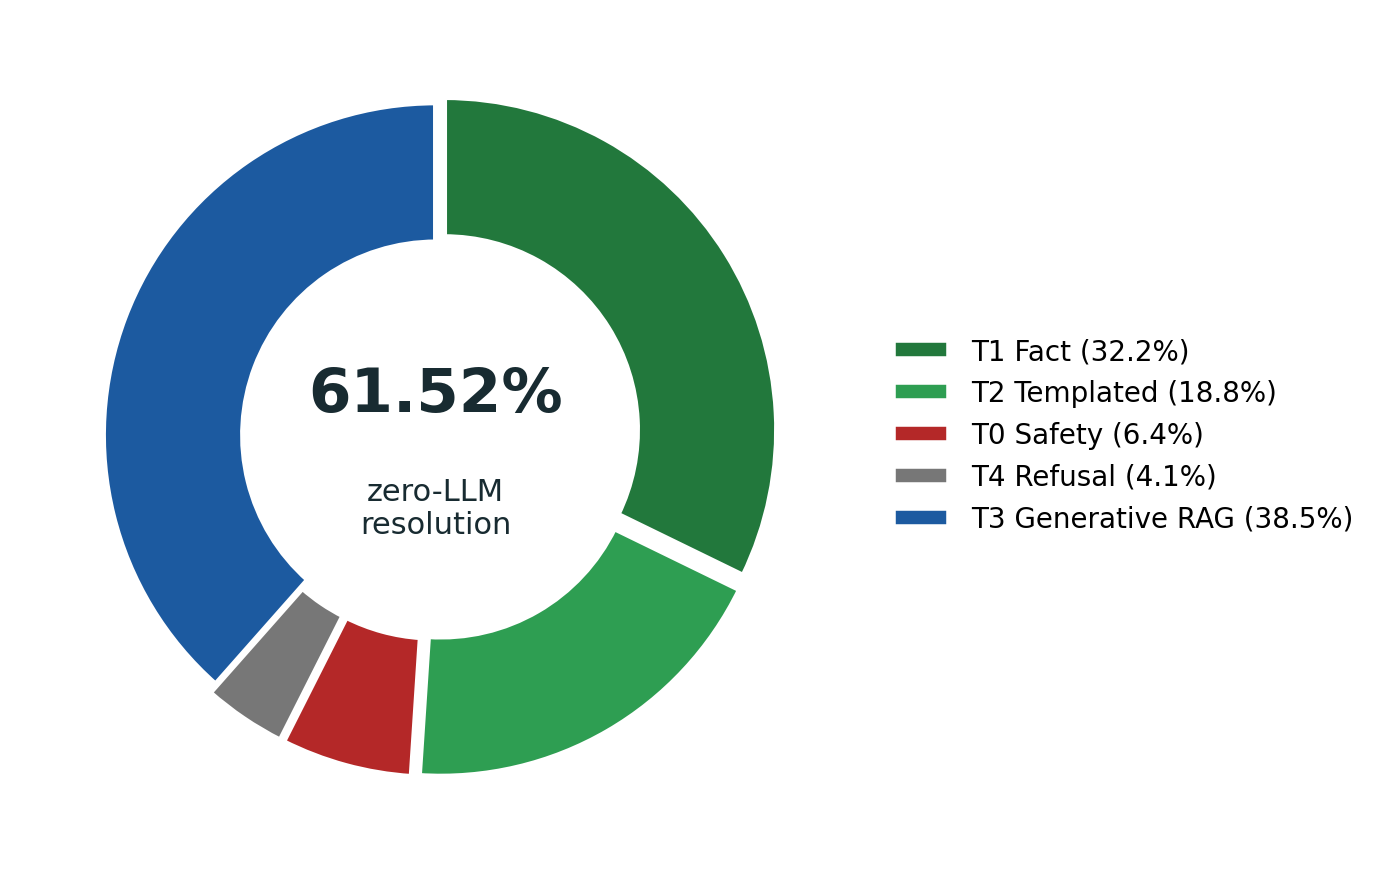
\includegraphics[width=0.78\textwidth]{figures/fig_3_tier_mix.png}
\vspace{-0.5em}
\caption{\textbf{E18 terminal-path mix.} The 61.52\% zero-LLM share includes deterministic advisory paths, safety handling, and refusal. The figure does not imply that every zero-LLM terminal produces an agronomically correct answer.}
\label{fig:tiermix}
\vspace{-0.5em}
\end{figure}

The proposed arm's weighted mean latency is 546.15 ms versus 1{,}247.93 ms for the comparison arm, a 2.28-fold ratio under the E18 model. Its modeled cost is \$0.0767 per 1{,}000 queries. The latency and cost results describe the harness and its assumptions; they are not a claim that all zero-LLM paths complete on a physical handset.

\subsection{RQ1 --- Deterministic Graph and Intent Components}
\label{subsec:e19}
E19 tests a small graph containing 23 nodes, 36 edges, and nine canonical facts across five target pairs. The reported 3-hop traversal produced 100\% slot completeness and 100\% provenance traceability at 0.0195 ms p95. This is evidence for the mechanism on the evaluated graph, not coverage of the full agricultural domain.

E25 exposes the principal component trade-off. On a generated/labeled dataset split into 4{,}500 training, 250 development, and 250 test examples, the 1.25 MB character $n$-gram classifier reached 96.4\% crop accuracy, 78.4\% pest accuracy, 100.0\% intent-type accuracy, and 78.4\% joint exact match. Its latency was 0.3855 ms p50 and 0.6719 ms p95. The comparison LLM had 94.2\% joint accuracy and 1{,}250 ms p50 in the artifact. The classifier is therefore smaller and faster, but less accurate on joint parsing; the downstream contract must absorb this error rather than the paper hiding it.

\subsection{RQ4 --- Network and Cache Behavior}
\label{subsec:e14}
E14 is a simulation of four network profiles over 1{,}000 queries, not a carrier or field trial. The result artifact reports 91.4\% cache delivery versus 82.0\% cloud-only at 15\% packet loss, and 58.1\% versus 12.8\% at 30\% packet loss. It also reports zero stale-advisory violations in the tested scenario. Because the claim ledger and master summary contain conflicting 30\%-loss values, these numbers are retained here as artifact readings pending reconciliation and are not used for a pooled safety or deployment claim.

\begin{figure}[t]
\centering
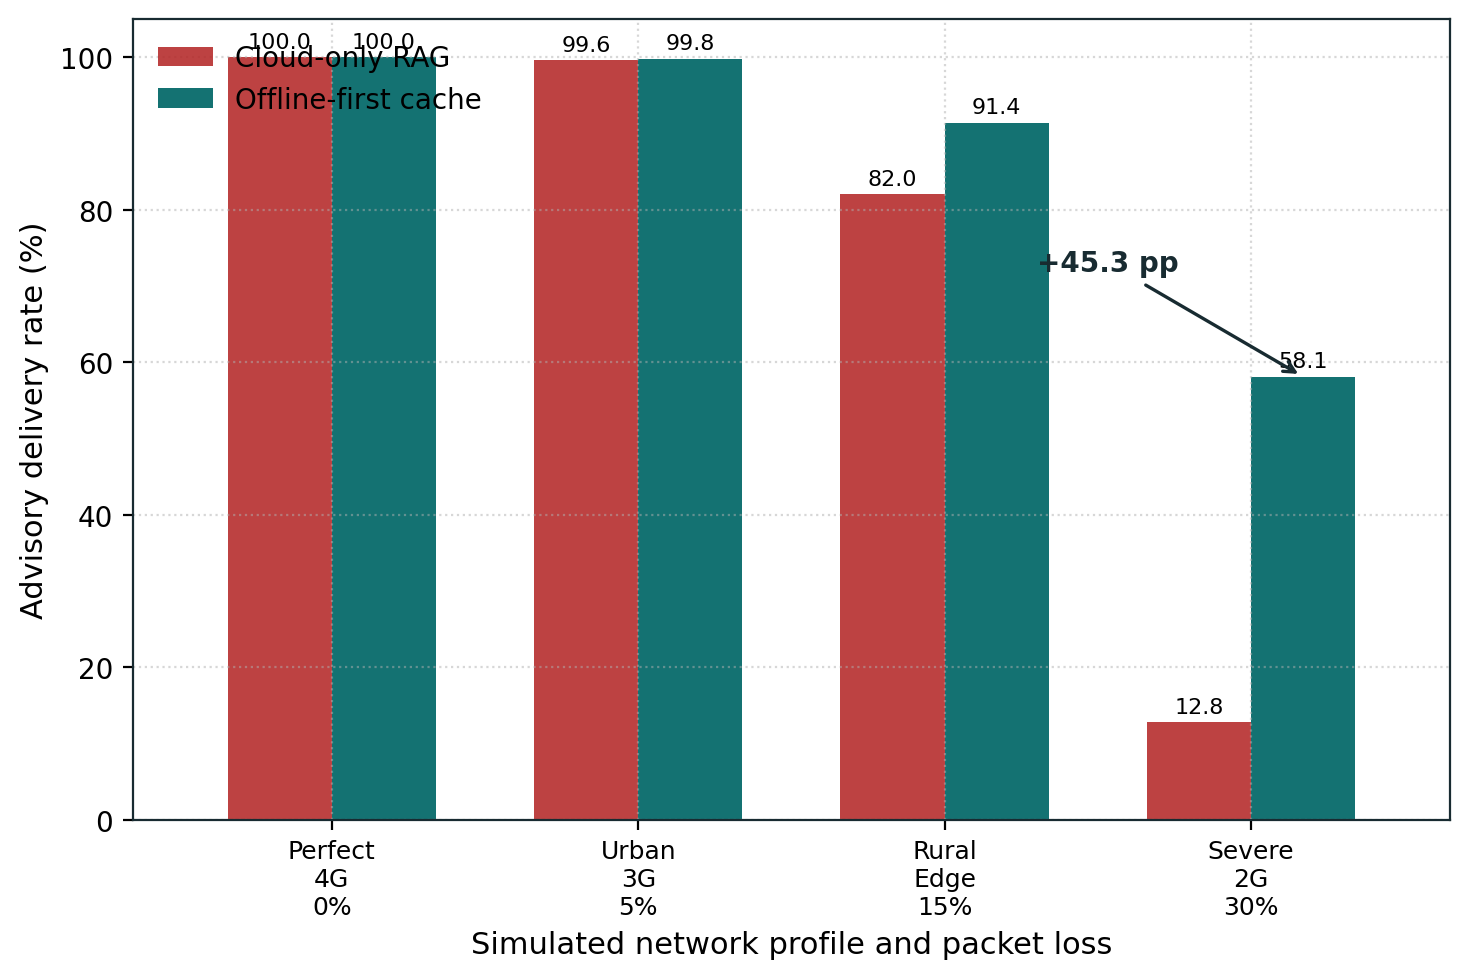
\includegraphics[width=0.80\textwidth]{figures/fig_4_network.png}
\vspace{-0.5em}
\caption{\textbf{E14 simulated delivery.} Profile labels and packet-loss rates are explicit. Values are emulator results; they are not measurements of a live rural carrier network.}
\label{fig:network}
\vspace{-0.5em}
\end{figure}

E23 tests 1{,}000 single-bit, record-swap, and deletion mutations against a SHA-256 hash-chained pack. The artifact reports 1{,}000/1{,}000 mutations detected, a 791-byte delta versus a 10{,}985-byte full pack, and 0.1919 ms p95 client verification latency. We report the zero-surviving-deprecated-record observation from the self-check, not the contradictory completeness percentage in the YAML.

\subsection{RQ5 --- GSM Composition and Injection Survivability}
\label{subsec:e15}
E15 evaluates 1{,}000 certified tuples. The deterministic template produced 102--115 GSM characters and preserved all selected dosage, interval, and PHI fields in the tested tuples. The LLM-composed arm had a 64.4\% critical-hazard rate, defined by omission or truncation of essential dosage/PHI constraints. This is a composition result, not live SMS delivery evidence.

E22 evaluates 1{,}400 adversarial payloads across the specified outbound-SMS attack families. The deterministic template leaked 0/1{,}400 payloads (95\% Wilson upper bound 0.27\%), while the LLM-composed arm leaked 509/1{,}400 (36.36\%). The endpoint is injection survivability into outbound SMS; it does not establish immunity for every chat or network attack.

\begin{figure}[t]
\centering
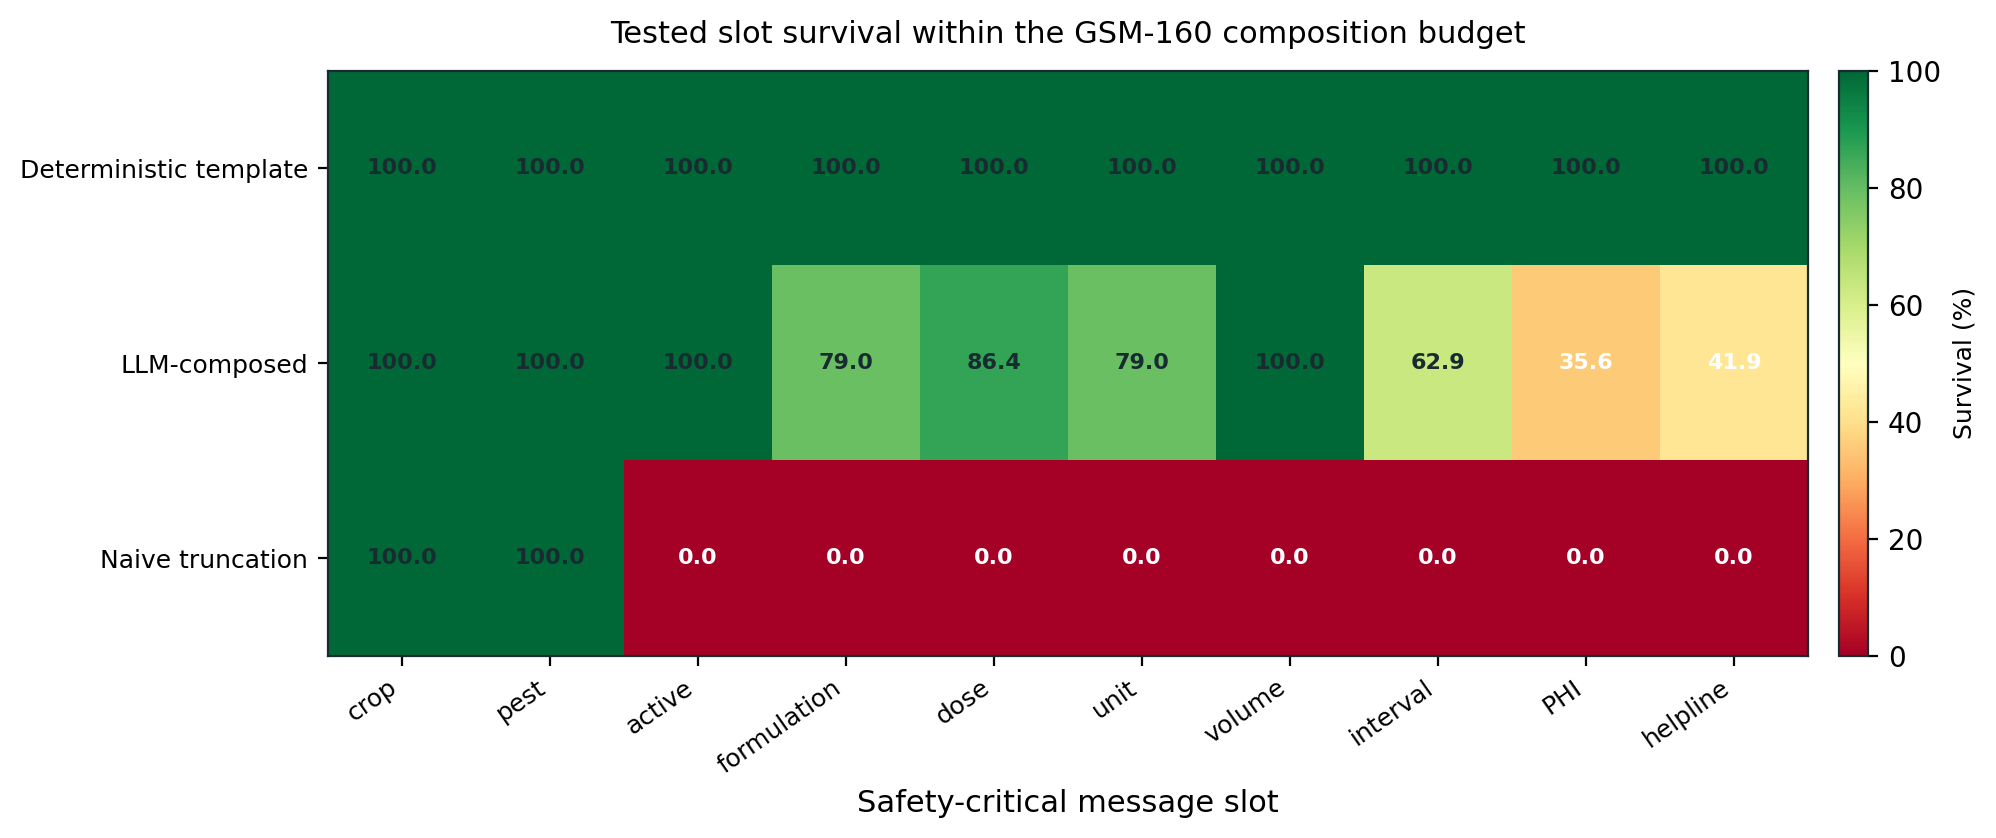
\includegraphics[width=\textwidth]{figures/fig_5_sms_slots.png}
\vspace{-0.5em}
\caption{\textbf{E15 tested slot survival.} The deterministic template preserves the selected slots in the evaluated tuples. The LLM and naive rows are controls from the same composition test; values describe field survival, not live-message delivery.}
\label{fig:sms_slots}
\vspace{-0.5em}
\end{figure}

\subsection{RQ3 --- Safety Stress Tests and Expert Review}
\label{subsec:safety_invariance}
The core safety artifacts report zero observed dangerous acceptance in their specified suites, including E02 relational misbinding, E03 slot ablation, E05 counterfactual binding, E07/E08 injection tests, and E11/E12 robustness layers. E02 reports 10{,}000/10{,}000 adversarial misbindings detected, while E03 reports the largest hazard increase when dosage bounds are removed. E13 contributes a human review of 200 responses by three agronomists, with Gwet's $\text{AC}_1=0.862$, mean correctness 4.82/5, and 96.5\% deployment approval in its artifact.

These are separate suites rather than a full factorial experiment over generator, retrieval corruption, dialect, classifier error, network state, cache state, and channel. A zero count is therefore an observed result conditional on each test set. The relevant interpretation is ``no dangerous acceptance observed under the specified test construction,'' not a universal zero-risk guarantee.

\subsection{RQ6 --- Scenario Economics and Knowledge Maintenance}
\label{subsec:e20}
E20 is an analytical scenario using 1 USD=120 BDT, a 0.25 BDT A2P SMS assumption, $0.00018$ per-query hosting amortization, the E18 tier fraction, six queries per farmer per year, and a 50\% online/30\% offline/20\% SMS channel mix. Its metrics block reports $0.0308$ BDT per online tiered query and a 2.86 versus 0.69 Crore BDT national scenario, but other project summaries report different totals. We therefore treat the national savings number as provisional until the price source, units, and ledger entry are reconciled.

E24 provides a narrower operational observation: authoring two BARI-verified facts for the Chili Anthracnose cluster in 18 minutes closed the evaluated 55-query gap, increased the measured sample's coverage from 58.7\% to 64.2\%, and yielded 3.06 newly resolvable queries per authoring minute. This rate belongs to that intervention; it is not a general authoring productivity law. E26 is exploratory and offline-only: three zero-source cases were recovered through the chunk fallback, with live LLM-side hazard testing still absent.


% -------------------------------------------------------------------------
% 7. FAILURE TAXONOMY
% -------------------------------------------------------------------------
\section{Failure Taxonomy}
\label{sec:failure_taxonomy}

A fail-closed design converts many uncertainty states into refusals, so evaluation must show where the system loses coverage and whether harmful candidates pass the tested boundary. Table~\ref{tab:failure_taxonomy} distinguishes measured failure modes from architectural dispositions.

\begin{table}[t]
\centering
\small
\caption{\textbf{Failure taxonomy.} The table records the intended disposition and measured scope. Zero observed dangerous acceptance is not a universal guarantee.}
\label{tab:failure_taxonomy}
\begin{tabularx}{\textwidth}{@{} L{3.4cm} L{2.3cm} Y c @{}}
\toprule
\textbf{Failure mode} & \textbf{Disposition} & \textbf{Effect \& mitigation} & \textbf{Layer} \\
\midrule
Detection below $\gamma$ or misclassification & Fall back to text & Routing loss; 3.15\% misrouting measured in E17 & E17 \\
Dialect or romanization variation & Text-first retrieval & Coverage endpoint, not correctness; 0.0\% observed hazard in E21 & E21 \\
Unbound safety slot & \textsc{Abstain} & Honest refusal + 16123 escalation & E7/E8 \\
Poisoned retrieval & \textsc{Abstain} & Single-record binding rejects fragments & E5 \\
Banned substance query & \textsc{Escalate} & Canned redirect to 16123 & E2 \\
Self-harm framing & \textsc{Escalate} & Supportive redirect + medical note & E2, E12 \\
Prompt injection & Filtered / \textsc{Abstain} & 0.0\% leakage (chat and SMS) & E12, E22 \\
Stale cached fact & Invalidated & Zero deprecated records survived the tested invalidation; 791\,B delta & E23 \\
Source-empty verification defect & Threat to validity & Captured production fallback once marked empty-source text as verified; not a safety result & Ledger S06 \\
Over-refusal (false abstain) & Coverage loss & Residual cases require expert escalation; workload not measured & E06/E21 \\
\bottomrule
\end{tabularx}
\vspace{-0.5em}
\end{table}

The principal operational cost of the fail-closed posture is \textbf{over-refusal}: a benign query may be withheld when the system cannot establish the required evidence relation. This protects the tested safety boundary at the cost of coverage and potential escalation demand. The project has not measured the resulting officer workload, so the paper treats that workload as an open deployment question rather than as a resolved benefit.

% -------------------------------------------------------------------------
% 8. DISCUSSION
% -------------------------------------------------------------------------
\section{Discussion}
\label{sec:discussion}

\subsection{What the Evaluations Support}
The results support a narrower systems conclusion. Metadata gating reduced the candidate search space and improved the tested Hit@1 and coverage endpoints, while the zero-LLM ladder reduced modeled latency and serving cost for the specified workload. Offline caching and deterministic GSM composition addressed separate delivery constraints in simulation and software tests. These gains are accompanied by costs: E17 reports 3.15\% misrouting, E25 reports 78.4\% joint classifier accuracy versus 94.2\% for the comparison LLM, 38.48\% of E18 traffic still reaches T3, and the E19 graph is small. The architecture therefore trades general language parsing capacity for bounded deterministic behavior and explicit fallback.

\subsection{Why the Contract Can Fail Closed}
The contract makes certification conditional on joint binding of the required slots to one evidence record. Under that contract, parser failure, missing evidence, contradiction, or an over-length SMS can lead to abstention rather than silent completion. The claim is conditional: it assumes correct extraction, authoritative and current records, no bypass, and an implementation that follows the contract. The separate stress suites recorded zero observed dangerous acceptances, but they do not establish a full factorial or population-wide safety guarantee.

\subsection{Deployment Implications}
The architecture suggests a deployment pathway in which DAE-approved records, local cache updates, GSM composition, and 16123 escalation are governed as one service boundary. That pathway remains a hypothesis because the study did not measure carrier delivery, referral follow-through, operator workload, or farmer outcomes. Transfer to veterinary, health, or disaster settings would require a new schema, evidence base, hazard taxonomy, and validation study.

% -------------------------------------------------------------------------
% 9. LIMITATIONS
% -------------------------------------------------------------------------
\section{Limitations and Threats to Validity}
\label{sec:limitations}

\textbf{Evidence status and reconciliation.} Several CEA-pivot YAMLs still record author acceptance as \texttt{PENDING}; E14, E20, and E25 contain conflicts across the YAML, ledger, or summary. Disputed values are not used in the abstract or pooled conclusion. \textbf{Simulated network conditions.} E14 uses a controlled emulator, not a live carrier network. \textbf{No physical profiling.} E16 is planned/blocked; there are no battery or thermal results. \textbf{Image and classifier limits.} E17 includes a bounded image/query-pairing construction and reports 3.15\% misrouting; E25 uses 5,000 generated/labeled samples and its joint accuracy trails the comparison LLM. \textbf{Fact-base scope.} E19 tests 23 nodes, 36 edges, nine facts, and five target pairs, not the whole domain. \textbf{Endpoint limits.} Coverage, Hit@1, slot completeness, and provenance are not agronomic correctness. E26 is offline-only and \texttt{done\_unverified}; live LLM-side hazard remains unmeasured. \textbf{Channel and economics.} E15/E22 test message strings, not carrier delivery; E20 is a scenario projection excluding device, training, support, maintenance, and escalation costs. \textbf{Outcomes.} No field trial, farmer study, yield measurement, poisoning measurement, trust study, or referral follow-through supports outcome claims. \textbf{Runtime boundary.} The captured production verifier and source-empty fallback defect must not be conflated with the research contract evaluated in the CEA layers.

% -------------------------------------------------------------------------
% 10. REPRODUCIBILITY
% -------------------------------------------------------------------------
\section{Reproducibility}
\label{sec:reproducibility}

Each layer has a specification, runner, raw output, and result artifact recorded through the acceptance protocol. The canonical trace is \texttt{experiments/registry.yaml}; its status fields distinguish completed, planned, blocked, and \texttt{done\_unverified} layers. The CEA layers use a limited derived dialect mapping, not the unrecoverable older 110-word map. No live retrieval or index construction occurs during the reported runs. Production assets are separated from research artifacts, and the application is not permitted to read the paper or experiment folders at runtime. Reproduction requires resolving the E14, E20, and E25 conflicts and recording author acceptance before submission.

% -------------------------------------------------------------------------
% 11. CONCLUSION
% -------------------------------------------------------------------------
\section{Conclusion}
\label{sec:conclusion}

This paper evaluated a bounded architecture for low-resource agricultural advisory. Structured metadata reduced the candidate search space, the tested ladder increased zero-LLM terminal handling, and deterministic cache and GSM components addressed specified network and message constraints. The fail-closed contract made refusal an explicit outcome, and the separate safety suites recorded zero observed dangerous acceptances within their stated constructions. Those findings support further validation; they do not establish universal safety, dialect immunity, field performance, national deployment readiness, or farmer benefit. The next decisive tests are physical-device profiling, carrier-level delivery, a live chunk-fallback lane, independent agronomic correctness labels per tier, and field-like evaluation of escalation and outcomes.

% -------------------------------------------------------------------------
% REFERENCES
% -------------------------------------------------------------------------
\bibliographystyle{plain}
\bibliography{references}

\end{document}
